\documentclass[letterpaper,11pt]{article}
\usepackage{latexsym}
\usepackage[empty]{fullpage}
\usepackage[usenames,dvipsnames]{color}
\usepackage{verbatim}
\usepackage{hyperref}
\usepackage{framed}
\usepackage{tocloft}
\usepackage{bibentry}
\usepackage{amsmath}
\usepackage{scrextend}
\usepackage{listings}
\usepackage{color}
\usepackage{fancyhdr}
\usepackage{graphicx}

%THIS PORTION IS FOR ADDING PAGE NUMBER
\pagestyle{fancy}
\cfoot{}
\rfoot{\thepage}
\renewcommand{\headrulewidth}{0pt}

%THIS PORTION IS FOR ADDING PAGE NUMBER
\urlstyle{same}
\definecolor{mygrey}{gray}{.85}
\definecolor{mygreylink}{gray}{.30}
\textheight=9.0in
\raggedbottom
\raggedright
\setlength{\tabcolsep}{0in}

%The following part is for inserting codes in LaTeX:
\definecolor{codegreen}{rgb}{0,0.6,0}
\definecolor{codegray}{rgb}{0.5,0.5,0.5}
\definecolor{codepurple}{rgb}{0.58,0,0.82}
\definecolor{backcolour}{rgb}{0.95,0.95,0.92}

\lstdefinestyle{mystyle}{
    backgroundcolor=\color{backcolour},
    commentstyle=\color{codegreen},
    keywordstyle=\color{magenta},
    numberstyle=\tiny\color{codegray},
    stringstyle=\color{codepurple},
    basicstyle=\footnotesize,
    breakatwhitespace=false,
    breaklines=true,
    captionpos=b,
    keepspaces=true,
    numbers=left,
    numbersep=5pt,
    showspaces=false,
    showstringspaces=false,
    showtabs=false,
    tabsize=2}
\lstset{style=mystyle}

% Adjust margins
\usepackage[left=0.9in,top=0.7in,right=0.9in,bottom=0.7in]{geometry}

% For centering elements in the tabular form
% http://bit.ly/2mtyAps
\usepackage{array}
\newcolumntype{P}[1]{>{\centering\arraybackslash}p{#1}}

%%%%%%%%%%%%%%%%%%%%%%%%%%%%%%%%%%%%%
%%%%%%   settings end here   %%%%%%%%
%%%%%%%%%%%%%%%%%%%%%%%%%%%%%%%%%%%%%

\begin{document}

\begin{center}
	\textbf{\Huge{Advanced Data Analysis HW6}}
\end{center}

\begin{center}
	\textsl{Ao Liu, al3472}
\end{center}

\bigbreak
\bigbreak
\bigbreak


%%%%%%%%%%%%%%%%%%%%%%%%%%%%%%%%%%%%%
%%%%%%%%%%%%%%   1   %%%%%%%%%%%%%%%%
%%%%%%%%%%%%%%%%%%%%%%%%%%%%%%%%%%%%%

\begin{addmargin}[-2em]{0em}
  \large{\textbf{1. }}
\end{addmargin}
\textbf{A random variable T is said to have a Weibull distribution is its survival function is give by $S(t) = e^{-(\alpha t)^\beta}$ where $\alpha > 0$ and $\beta > 0$.}

\begin{addmargin}[-1.1em]{0em}
  \textbf{(a)}\par
\end{addmargin}
\textbf{Find the density, $f_T (t)$ of T}\par
\bigbreak
\begin{addmargin}[-0.5em]{0em}
  \textbf{Answer: }
\end{addmargin}

$$f_T(t) = -\frac{dS(t)}{dt} = \beta\alpha^{\beta}t^{\beta-1}e^{-(\alpha t)^{\beta}}$$



\begin{addmargin}[-1.1em]{0em}
  \textbf{(b)}\par
\end{addmargin}
\textbf{Find the hazard function $\lambda(t)$ of T}\par
\bigbreak
\begin{addmargin}[-0.5em]{0em}
  \textbf{Answer: }
\end{addmargin}

$$\lambda(t) = \frac{f(t)}{S(t)} = \beta\alpha^{\beta}t^{\beta-1}$$


\begin{addmargin}[-1.1em]{0em}
  \textbf{(c)}\par
\end{addmargin}
\textbf{Show that}
$$log(-log(S(t))) = \beta log(\alpha) + \beta log(t)$$
\textbf{Based on this, describe a graphical method for checking whether or not the data is
from a Weibull distribution.}\par
\bigbreak
\begin{addmargin}[-0.5em]{0em}
  \textbf{Answer: }
\end{addmargin}

\begin{align}
log(-log(S(t))) & = log((\alpha t)^{\beta})\nonumber\\
& = \beta log(\alpha t) \nonumber\\
& = \beta log(\alpha) + \beta log(t) \nonumber
\end{align}

Here we get a graphical method for checking whether or not the data is from a Weibull distribution: By plotting all the $(log(t), log(-log(S(t))))$, the points from the same Weibull distribution should lie in a straight line.


\begin{addmargin}[-1.1em]{0em}
  \textbf{(d)}\par
\end{addmargin}
\textbf{Consider the following data}
$$143, 164, 188, 188, 190, 192, 206, 209, 213, 216, 220, 227, 230, 234, 246, 265, 304$$
\textbf{and use as an estimate of $S(t(i))$}
$$Sˆ(t(i)) = 1 − (i - 0.5)/n$$
\textbf{were $t(i)$ is the ith ordered value and n is the sample size. Use the graphical technique
in the previous question to check if a Weibull distribution is appropriate for these data}\par
\bigbreak
\begin{addmargin}[-0.5em]{0em}
  \textbf{Answer: }
\end{addmargin}

Follow the technique in (c), we plot all the $(log(t_i), log(-log(\hat{S}(t_i)))$ in an axis:
\begin{lstlisting}
> data = c(143, 164, 188, 188, 190, 192, 206, 209, 213, 216, 220, 227, 230, 234, 246, 265, 304)
> result = c()
> n = length(data)
> for (i in 1:17){
    result[i] = 1-(i-0.5)/n
  }
> plot(log(-log(result))~log(data))
> abline(lm(log(-log(result))~log(data)))
\end{lstlisting}

\begin{center} \makebox[\linewidth]{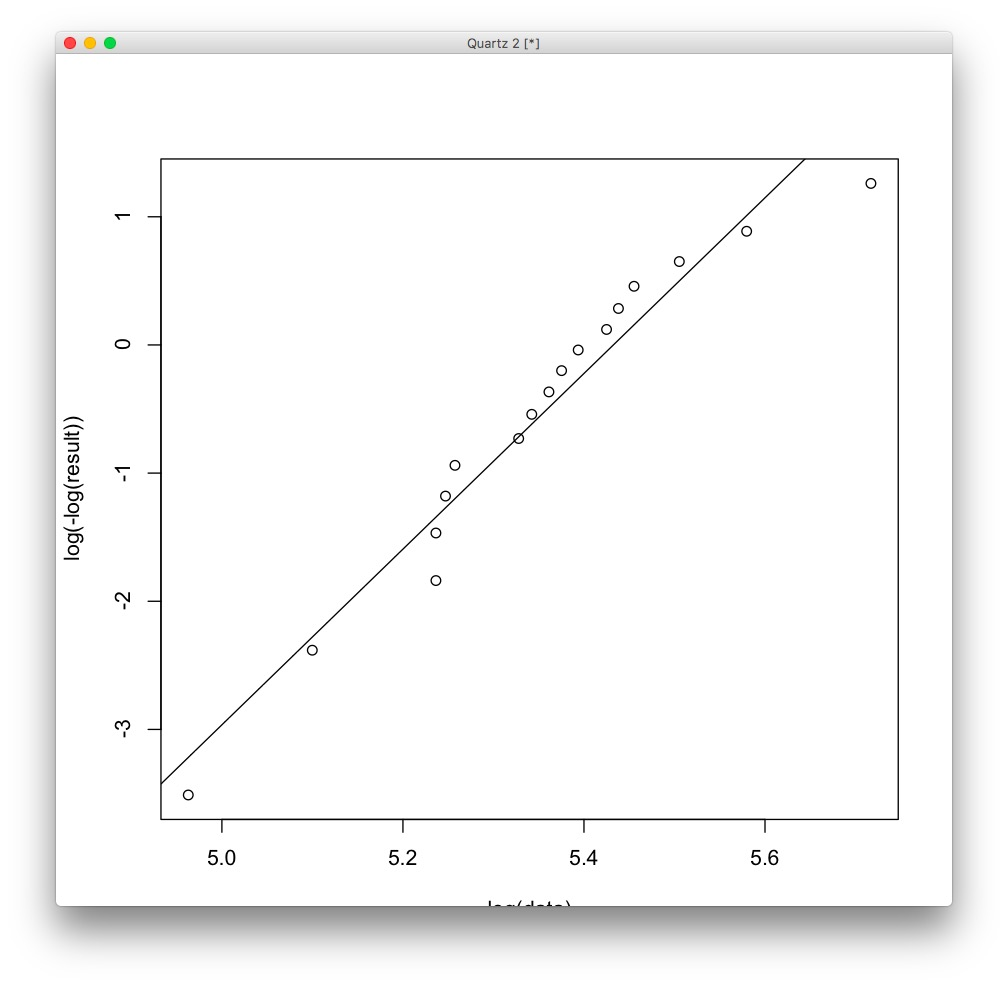
\includegraphics[width=\textwidth]{HW61.jpg}}
\end{center}
We can tell from the plot that a Weibull distribution is appropriate for these data.

\begin{addmargin}[-1.1em]{0em}
  \textbf{(e)}\par
\end{addmargin}
\textbf{Assume that the Weibull distribution is a good fit, use least squares approach to estimate its parameters.}\par
\bigbreak
\begin{addmargin}[-0.5em]{0em}
  \textbf{Answer: }
\end{addmargin}

\begin{lstlisting}
> fit = lm(log(-log(result))~log(data))
> abline(fit)
> summary(fit)
\end{lstlisting}

\begin{lstlisting}
  Call:
lm(formula = log(-log(result)) ~ log(data))

Residuals:
     Min       1Q   Median       3Q      Max
-0.68997 -0.12226  0.09174  0.19153  0.30116

Coefficients:
            Estimate Std. Error t value Pr(>|t|)
(Intercept) -37.2330     2.1806  -17.07 3.08e-11 ***
log(data)     6.8538     0.4073   16.83 3.80e-11 ***
---
Signif. codes:  0 ‘***’ 0.001 ‘**’ 0.01 ‘*’ 0.05 ‘.’ 0.1 ‘ ’ 1

Residual standard error: 0.2871 on 15 degrees of freedom
Multiple R-squared:  0.9497,	Adjusted R-squared:  0.9463
F-statistic: 283.1 on 1 and 15 DF,  p-value: 3.796e-11
\end{lstlisting}

Assume that the Weibull distribution is a good fit, by using least squares approach, we have the following estimation for its parameters:
$$ \beta = 6.8538$$
$$ \alpha = e^{\frac{-37.2330}{\beta}} = 0.0044$$




\begin{addmargin}[-2em]{0em}
  \large{\textbf{2. }}
\end{addmargin}
\textbf{The data below show survival times in months of patients with Hodgkin’s disease who were treated with nitrogen mustard. Group A patients received little or no prior therapy whereas Group B patients received heavy prior therapy. Starred are observations are censoring times.}\par

\begin{align}
GroupA : &1.25, 1.41, 4.98, 5.25, 5.38, 6.92, 8.89, 10.98, 11.18, 13.11, 13.21, 16.33, 19.77, \nonumber\\
  &21.08, 21.84^*, 22.07, 31.38, 32.61^*, 37.18^*, 42.92\nonumber
\end{align}
\begin{align}
GroupB : &1.05, 2.92, 3.61, 4.20, 4.49, 6.72, 7.31, 9.08, 9.11, 14.49^*, \nonumber\\
&16.85, 18.82^*, 26.59^*, 30.26^*, 41.34^*\nonumber
\end{align}

\begin{addmargin}[-1.1em]{0em}
  \textbf{(a)}\par
\end{addmargin}
\textbf{Obtain and plot the Kaplan Meier estimates of $S_A$ and $S_B$, the corresponding survival functions.}\par
\bigbreak
\begin{addmargin}[-0.5em]{0em}
  \textbf{Answer: }
\end{addmargin}

For group A, we have:
\begin{center}
\begin{tabular}{ P{2cm}P{1cm}P{1cm}P{1cm}P{1cm}P{1cm}P{1cm}P{1cm}P{1cm}P{1cm}P{1cm}P{1cm}P{1cm}P{1cm}P{1cm}P{1cm}P{1cm}}
$y_A(i)$ &1.25 &1.41 &4.98 &5.25 &5.38 &6.92 &8.89 &10.98 &11.18 &13.11 &13.21 &16.33 &19.77 &21.08 &22.07 &42.92\\
$d_A(i)$ &1 &1 &1 &1 &1 &1 &1 &1 &1 &1 &1 &1 &1 &1 &1 &1\\
$N_A(i)$ &20 &19 &18 &17 &16 &15 &14 &13 &12 &11 &10 &9 &8 &7 &5 &1\\
\end{tabular}
\end{center}

So the Kaplan-Meier estimator of S(t) is:
$$\hat{S}_A(t) & = \Pi_{y_A(j)\leq t}(1-\frac{d_A(j)}{N_A(j)})$$

For group B, we have:
\begin{center}
\begin{tabular}{ P{2cm}P{1cm}P{1cm}P{1cm}P{1cm}P{1cm}P{1cm}P{1cm}P{1cm}P{1cm}P{1cm}}
$y_B(i)$ &1.05 &2.92 &3.61 &4.20 &4.49 &6.72 &7.31 &9.08 &9.11 &16.85\\
$d_B(i)$ &1 &1 &1 &1 &1 &1 &1 &1 &1 &1\\
$N_B(i)$ &15 &14 &13 &12 &11 &10 &9 &8 &7 &5\\
\end{tabular}
\end{center}

So the Kaplan-Meier estimator of S(t) is:
$$\hat{S}_B(t) & = \Pi_{y_B(j)\leq t}(1-\frac{d_B(j)}{N_B(j)})$$


\begin{lstlisting}
> library(survival)
> time = c(1.25, 1.41, 4.98, 5.25, 5.38, 6.92, 8.89, 10.98, 11.18, 13.11, 13.21, 16.33, 19.77, 21.08, 21.84, 22.07, 31.38, 32.61, 37.18, 42.92, 1.05, 2.92, 3.61, 4.20, 4.49, 6.72, 7.31, 9.08, 9.11, 14.49, 16.85, 18.82, 26.59, 30.26, 41.34)
> status = c(1, 1, 1, 1, 1, 1, 1, 1, 1, 1, 1, 1, 1, 1, 0, 1, 0, 0, 0, 1, 1, 1, 1, 1, 1, 1, 1, 1, 1, 0, 1, 0, 0, 0, 0)
> group = c(1,1,1,1,1,1,1,1,1,1,1,1,1,1,1,1,1,1,1,1,2,2,2,2,2,2,2,2,2,2,2,2,2,2,2)
> fit <- survfit(Surv(time,status)~group,type = "kaplan-meier")
> plot(fit, lty=1:2 )
\end{lstlisting}


\begin{center} \makebox[\linewidth]{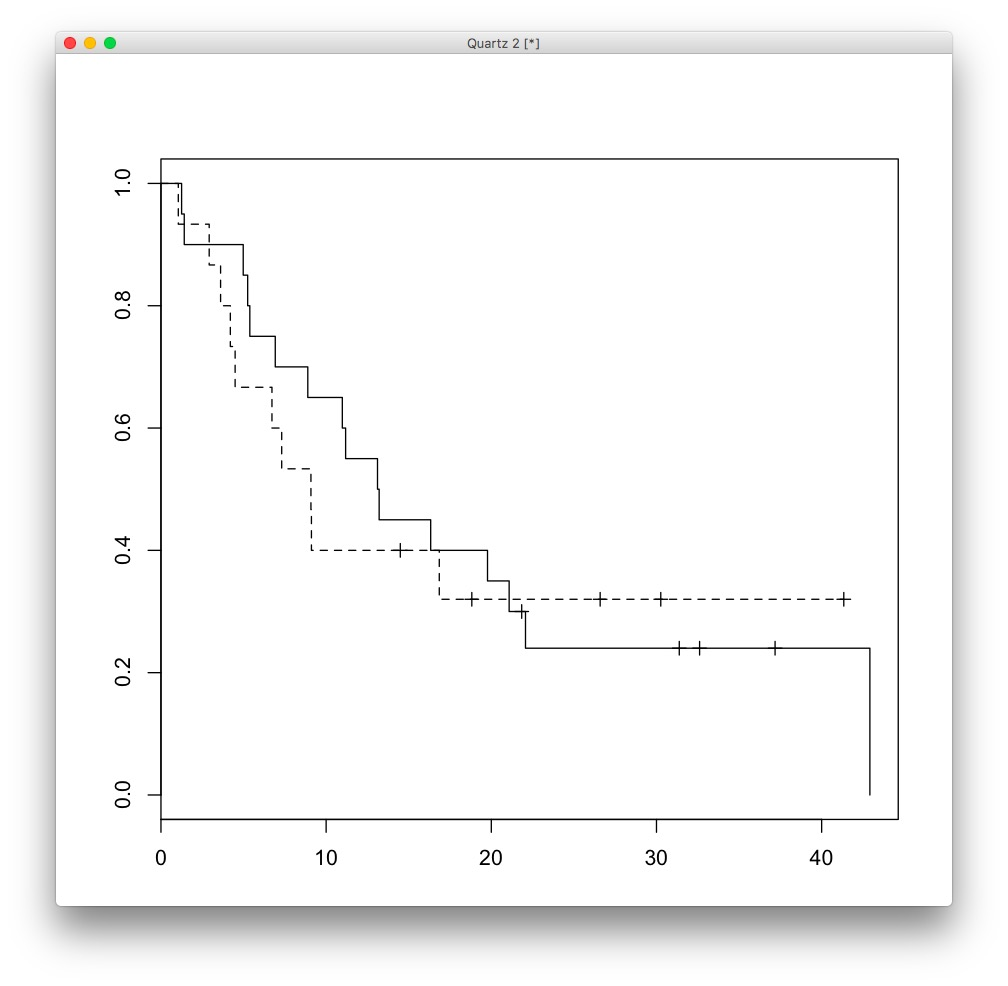
\includegraphics[width=\textwidth]{HW62.jpg}}
\end{center}

\begin{addmargin}[-1.1em]{0em}
  \textbf{(b)}\par
\end{addmargin}
\textbf{Estimate $S_A(10)$ and $S_B(10)$ using a 95\% confidence interval.}\par
\bigbreak
\begin{addmargin}[-0.5em]{0em}
  \textbf{Answer: }
\end{addmargin}


\begin{lstlisting}
> summary(fit)
\end{lstlisting}

\begin{lstlisting}
  Call: survfit(formula = Surv(time, status) ~ group, type = "kaplan-meier")

                group=1
  time n.risk n.event survival std.err lower 95% CI upper 95% CI
  1.25     20       1     0.95  0.0487        0.859        1.000
  1.41     19       1     0.90  0.0671        0.778        1.000
  4.98     18       1     0.85  0.0798        0.707        1.000
  5.25     17       1     0.80  0.0894        0.643        0.996
  5.38     16       1     0.75  0.0968        0.582        0.966
  6.92     15       1     0.70  0.1025        0.525        0.933
  8.89     14       1     0.65  0.1067        0.471        0.897
 10.98     13       1     0.60  0.1095        0.420        0.858
 11.18     12       1     0.55  0.1112        0.370        0.818
 13.11     11       1     0.50  0.1118        0.323        0.775
 13.21     10       1     0.45  0.1112        0.277        0.731
 16.33      9       1     0.40  0.1095        0.234        0.684
 19.77      8       1     0.35  0.1067        0.193        0.636
 21.08      7       1     0.30  0.1025        0.154        0.586
 22.07      5       1     0.24  0.0980        0.108        0.534
 42.92      1       1     0.00     NaN           NA           NA

                group=2
  time n.risk n.event survival std.err lower 95% CI upper 95% CI
  1.05     15       1    0.933  0.0644        0.815        1.000
  2.92     14       1    0.867  0.0878        0.711        1.000
  3.61     13       1    0.800  0.1033        0.621        1.000
  4.20     12       1    0.733  0.1142        0.540        0.995
  4.49     11       1    0.667  0.1217        0.466        0.953
  6.72     10       1    0.600  0.1265        0.397        0.907
  7.31      9       1    0.533  0.1288        0.332        0.856
  9.08      8       1    0.467  0.1288        0.272        0.802
  9.11      7       1    0.400  0.1265        0.215        0.743
 16.85      5       1    0.320  0.1239        0.150        0.684
\end{lstlisting}


According to the output from above,
$$\hat{S}_A(10) = \hat{S}_A(8.89) = 0.65$$
the 95\% CI for $\hat{S}_A(10)$ is:
$$(0.471, 0.897)$$
$$\hat{S}_B(10) = \hat{S}_B(9.11) = 0.40$$
the 95\% CI for $\hat{S}_B(10)$ is:
$$(0.215,0.743)$$



\begin{addmargin}[-1.1em]{0em}
  \textbf{(c)}\par
\end{addmargin}
\textbf{Test $H_0$ :$S_A$ =$S_B$ against $H_a$ :$S_A \neq S_B$. Use $\alpha=0.05$.}\par
\bigbreak
\begin{addmargin}[-0.5em]{0em}
  \textbf{Answer: }
\end{addmargin}
To test the hypothesis, we do the following test in R:
\begin{lstlisting}
> survdiff(Surv(time,status)~group, rho=0)
\end{lstlisting}

\begin{lstlisting}
  Call:
survdiff(formula = Surv(time, status) ~ group, rho = 0)

         N Observed Expected (O-E)^2/E (O-E)^2/V
group=1 20       16    16.66    0.0261    0.0749
group=2 15       10     9.34    0.0466    0.0749

 Chisq= 0.1  on 1 degrees of freedom, p= 0.784
\end{lstlisting}
Since the p-value is $0.784 > 0.05$, we cannot reject the Null Hypothesis that $S_A = S_B$.


\end{document}

%%%%%%%%%%%%%%%%%%%%%%%%%%%%%%%%%%%%%
%%%%%%%%%%%%%%   #   %%%%%%%%%%%%%%%%
%%%%%%%%%%%%%%%%%%%%%%%%%%%%%%%%%%%%%

%Insert pics:
%%%%%%%%%%%%%
%\begin{center}
  %\makebox[\linewidth]{\includegraphics[width=\textwidth]{4640HW6.jpg}}
%\end{center}

%insert a complicated tab...
%%%%%%%%%%%%%%%%%%%%%%%%%%%%
%\begin{center}
%\begin{tabular}{ P{12cm}P{1cm}P{1cm}P{1cm}  }
%& \multicolumn{3}{c}{Posterior Quantiles} \\
%\centering{Quantity of Interest} & 25\% & 50\% & 75\% \\
%\hline
%geometric mean for Blue Earth (no basement), exp($\beta_2)$ &4.1& 5.0& 6.5\\
%geometric mean for Blue Earth County (basement), exp($\beta_1+\beta_2)$ &6.1 &7.1 &8.2\\
%geometric mean for Clay County (no basement), exp($\beta_3)$& 3.8& 4.7 &5.8\\
%geometric mean for Clay County (basement), exp($\beta_1+\beta_3)$ &5.6& 6.5& 7.6\\
%geometric mean for Goodhue County (no basement), exp($\beta_4)$ & 3.9 &4.9& 6.2\\
%geometric mean for Goodhue County (basement), exp($\beta_1+\beta_4)$ &5.8& 6.8& 7.9\\
%factor for basement vs. no basement, exp($\beta_1$)&1.1& 1.4 &1.7\\
%geometric sd of predictions, exp($\sigma$)&2.1 &2.2& 2.4\\
%\end{tabular}
%\end{center}

% simple version:
% The capital P is defined in the header
% \begin{center}
% \begin{tabular}{ P{1cm}P{1cm}P{1cm}P{1cm}P{1cm}P{1cm}}
% {} & 1 & 2 & 3 & 4 & 5 \\
% \hline
% 1 &1,1 &0,0 &0,0 &0,0 &0,0\\
% 2 &0,0 &1,1 &0,0 &0,0 &0,0\\
% 3 &0,0 &0,0 &1,1 &0,0 &0,0\\
% 4 &0,0 &0,0 &0,0 &1,1 &0,0\\
% 5 &0,0 &0,0 &0,0 &0,0 &1,1\\
% \end{tabular}
% \end{center}

%%%insert code snippets:
%%%%%%%%%%%%%%%%%%%%%%%%
%\begin{lstlisting}
%INSERT CODE HERE
%\end{lstlisting}

%%insert equation with severl lines:
%\begin{align}
%LEFT &= RIGHT1 \nonumber\\
%     &= RIGHT2 \nonumber\\
%     &= RIGHT3 \nonumber
%\end{align}

%insert a 大括号...
% $$ leftside = \begin{cases}
%   case1 & detail1 \\
%   case2 & detail2 \\
%   case3 & detail3
% \end{cases}$$

% insert text under equation mode:
% \textrm{the text that you need}

% inset a space:
% \:

%ssh-add ~/.ssh/id_rsa
